\documentclass{article}
\usepackage[utf8]{inputenc}
\usepackage{amsmath}
\usepackage{amsfonts}
\usepackage{amssymb}
\usepackage{graphicx}
\usepackage{indentfirst}
\usepackage{listings}
\usepackage{xcolor}
\usepackage{fancyhdr} % permet de creer des entetes et pieds de page
\usepackage{float}

% Configuration de l'en-tête et du pied de page
\pagestyle{fancy}
\fancyhf{}
\lhead{Sanna Thomas}
\rhead{L3 STI}
\chead{Rapport Exo 1 Seance 5}
\rfoot{Page n°\thepage}

\begin{document}

\begin{titlepage}
  \title{TD Seance 5: Exercice 1 Wireshark}
  \author{SANNA Thomas}
  \date{\today}
  \maketitle
\end{titlepage}

\section*{Question 3}

Après avoir ouvert Firefox, et ensuite avoir lancé une écoute Wireshark, lorsque l'on ouvre le lien dans https://random.dog/woof.json, on peut voir que l'on envoie et reçois des paquets de type TCP.

\begin{figure}[H]
  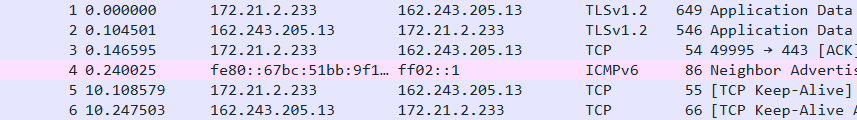
\includegraphics[width=\linewidth]{resRandomDog.png}
  \caption{Capture de paquets}
  \label{fig:resRandomDog}
\end{figure}

\section*{Question 4}

Plusieurs protocoles sont utilisés pour la communication:

\begin{itemize}
  \item TCP
  \item TLSv1.2
  \item ICMPV6
  \item HTTP ne semble pas être utilisé
\end{itemize}

\section*{Question 5}

Les protocoles dont le paquet contient l'adresse IP du serveur est le protocole ICMPV6 (IPV6) et le protocole TCP (IPV4).

\section*{Question 6}

Les protocoles utilisés pour l'envoi de données sont le protocole TCP et le protocole TLSv1.2.

\begin{figure}[H]
  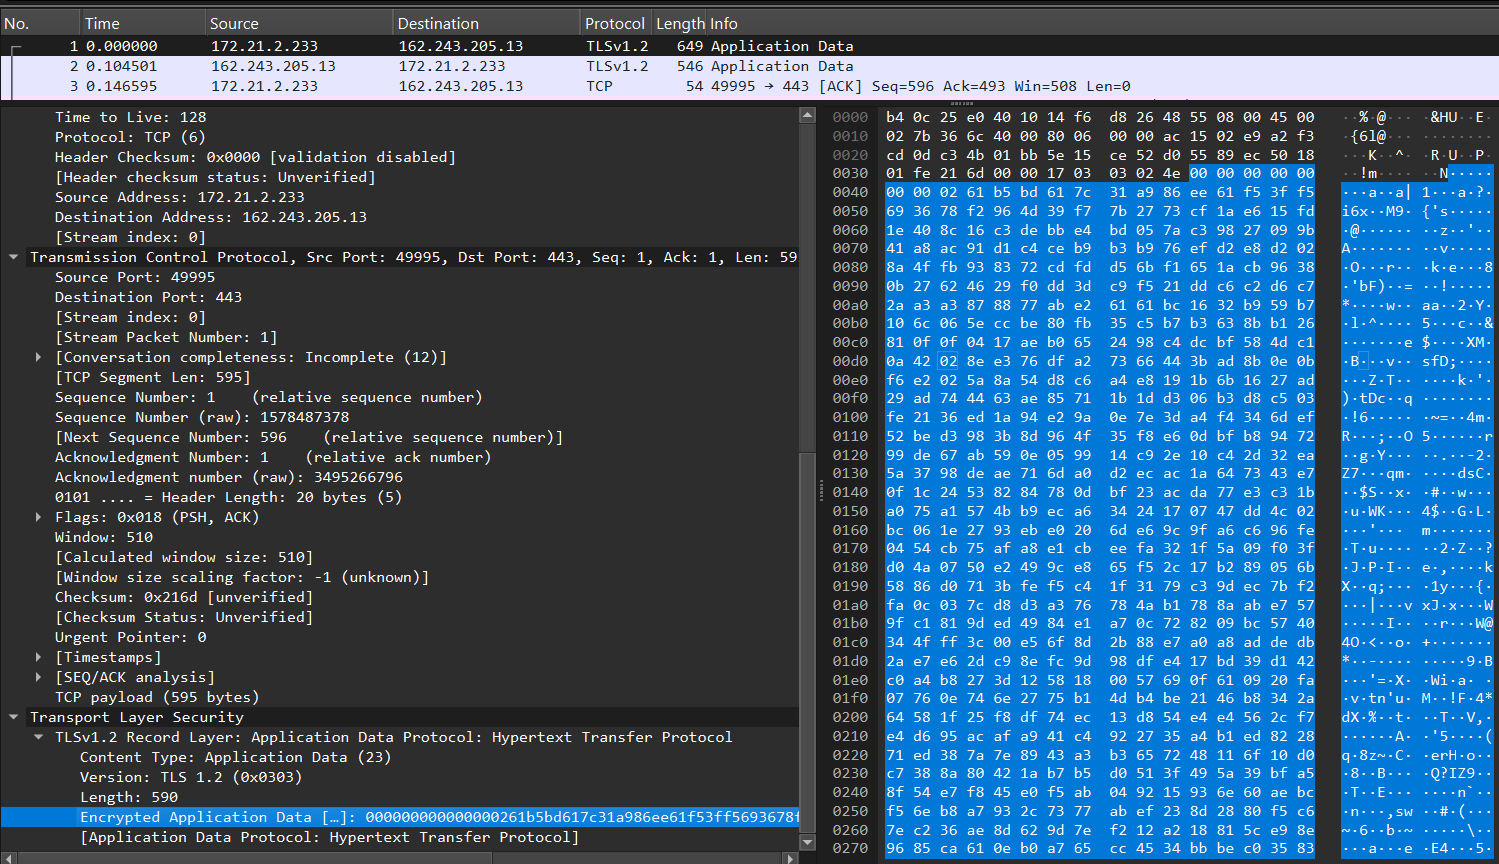
\includegraphics[width=\linewidth]{envoiData.png}
  \caption{Capture de paquets}
  \label{fig:resRandomDog2}
\end{figure}


\end{document}